% Template adapted from https://github.com/jgm/pandoc-templates/blob/master/default.latex
% To be used with XeLaTex in memoiR
%%%%%%%%%%%%%%%%%%%%%%%%%%%%%%%%%%%%%%%%%%%%%%%%%%%%%%%%%%%%%%%%%%%%%%%%%%%%%%%%%%%%%%%%%

% Options for packages loaded elsewhere
\PassOptionsToPackage{unicode=true}{hyperref}
\PassOptionsToPackage{hyphens}{url}
\PassOptionsToPackage{dvipsnames,svgnames*,x11names*}{xcolor}
% Right to left support


\documentclass[
  10pt,
  italian,
  a4paper,
  extrafontsizes,onecolumn,openright
  ]{memoir}

% Double (or whatever) spacing

% Math
\usepackage{amssymb, amsmath}
% mathspec: arbitrary math fonts
\usepackage{unicode-math}
\defaultfontfeatures{Scale=MatchLowercase}
\defaultfontfeatures[\rmfamily]{Ligatures=TeX,Scale=1}

% Fonts
% \usepackage{lmodern}
\usepackage{fontspec}

% Main font
% Specific sanserif font
% Specific monotype font
\setmonofont[Scale=0.75]{Operator Mono SSm Book}
% Specific math font
% Chinese, Japanese, Corean fonts

% Use upquote for straight quotes in verbatim environments
\usepackage{upquote}
% Use microtype
\usepackage[]{microtype}
\UseMicrotypeSet[protrusion]{basicmath} % disable protrusion for tt fonts

% Verbatim in note

% Color links
\usepackage{xcolor}

% Strikeout

% Necessary for code chunks
\usepackage{color}
\usepackage{fancyvrb}
\newcommand{\VerbBar}{|}
\newcommand{\VERB}{\Verb[commandchars=\\\{\}]}
\DefineVerbatimEnvironment{Highlighting}{Verbatim}{commandchars=\\\{\}}
% Add ',fontsize=\small' for more characters per line
\newenvironment{Shaded}{}{}
\newcommand{\AlertTok}[1]{\textcolor[rgb]{1.00,0.00,0.00}{\textbf{#1}}}
\newcommand{\AnnotationTok}[1]{\textcolor[rgb]{0.38,0.63,0.69}{\textbf{\textit{#1}}}}
\newcommand{\AttributeTok}[1]{\textcolor[rgb]{0.49,0.56,0.16}{#1}}
\newcommand{\BaseNTok}[1]{\textcolor[rgb]{0.25,0.63,0.44}{#1}}
\newcommand{\BuiltInTok}[1]{#1}
\newcommand{\CharTok}[1]{\textcolor[rgb]{0.25,0.44,0.63}{#1}}
\newcommand{\CommentTok}[1]{\textcolor[rgb]{0.38,0.63,0.69}{\textit{#1}}}
\newcommand{\CommentVarTok}[1]{\textcolor[rgb]{0.38,0.63,0.69}{\textbf{\textit{#1}}}}
\newcommand{\ConstantTok}[1]{\textcolor[rgb]{0.53,0.00,0.00}{#1}}
\newcommand{\ControlFlowTok}[1]{\textcolor[rgb]{0.00,0.44,0.13}{\textbf{#1}}}
\newcommand{\DataTypeTok}[1]{\textcolor[rgb]{0.56,0.13,0.00}{#1}}
\newcommand{\DecValTok}[1]{\textcolor[rgb]{0.25,0.63,0.44}{#1}}
\newcommand{\DocumentationTok}[1]{\textcolor[rgb]{0.73,0.13,0.13}{\textit{#1}}}
\newcommand{\ErrorTok}[1]{\textcolor[rgb]{1.00,0.00,0.00}{\textbf{#1}}}
\newcommand{\ExtensionTok}[1]{#1}
\newcommand{\FloatTok}[1]{\textcolor[rgb]{0.25,0.63,0.44}{#1}}
\newcommand{\FunctionTok}[1]{\textcolor[rgb]{0.02,0.16,0.49}{#1}}
\newcommand{\ImportTok}[1]{#1}
\newcommand{\InformationTok}[1]{\textcolor[rgb]{0.38,0.63,0.69}{\textbf{\textit{#1}}}}
\newcommand{\KeywordTok}[1]{\textcolor[rgb]{0.00,0.44,0.13}{\textbf{#1}}}
\newcommand{\NormalTok}[1]{#1}
\newcommand{\OperatorTok}[1]{\textcolor[rgb]{0.40,0.40,0.40}{#1}}
\newcommand{\OtherTok}[1]{\textcolor[rgb]{0.00,0.44,0.13}{#1}}
\newcommand{\PreprocessorTok}[1]{\textcolor[rgb]{0.74,0.48,0.00}{#1}}
\newcommand{\RegionMarkerTok}[1]{#1}
\newcommand{\SpecialCharTok}[1]{\textcolor[rgb]{0.25,0.44,0.63}{#1}}
\newcommand{\SpecialStringTok}[1]{\textcolor[rgb]{0.73,0.40,0.53}{#1}}
\newcommand{\StringTok}[1]{\textcolor[rgb]{0.25,0.44,0.63}{#1}}
\newcommand{\VariableTok}[1]{\textcolor[rgb]{0.10,0.09,0.49}{#1}}
\newcommand{\VerbatimStringTok}[1]{\textcolor[rgb]{0.25,0.44,0.63}{#1}}
\newcommand{\WarningTok}[1]{\textcolor[rgb]{0.38,0.63,0.69}{\textbf{\textit{#1}}}}

% Listings package

% Tables
\usepackage{longtable,booktabs,tabu}
% Fix footnotes in tables (requires footnote package)
\IfFileExists{footnote.sty}{\usepackage{footnote}\makesavenoteenv{longtable}}{}

% Graphics
\usepackage{graphicx,grffile}
\graphicspath{{images/}}
\makeatletter
\def\maxwidth{\ifdim\Gin@nat@width>\linewidth\linewidth\else\Gin@nat@width\fi}
\def\maxheight{\ifdim\Gin@nat@height>\textheight\textheight\else\Gin@nat@height\fi}
\makeatother
% Scale images if necessary, so that they will not overflow the page
% margins by default, and it is still possible to overwrite the defaults
% using explicit options in \includegraphics[width, height, ...]{}
\setkeys{Gin}{width=\maxwidth,height=\maxheight,keepaspectratio}

% Prevent overfull lines
\setlength{\emergencystretch}{3em}  
\providecommand{\tightlist}{%
  \setlength{\itemsep}{0pt}\setlength{\parskip}{0pt}}

% Number sections for memoir (secnumdepth counter is ignored)
\setsecnumdepth{section}

% Set default figure placement to htbp
\makeatletter
\def\fps@figure{htbp}
\makeatother

% Spacing in lists
\usepackage{enumitem}

% Polyglossia
\usepackage{polyglossia}
\setmainlanguage{it}
\setotherlanguage{en-US}

% BibLaTeX
\usepackage[backend=biber,style=authoryear-ibid,isbn=false,backref=true,giveninits=true,uniquename=init,maxcitenames=2,maxbibnames=150,sorting=nyt,sortcites=false,style=apa]{biblatex}
\addbibresource{refs.bib}
\addbibresource{packages.bib}

% cslreferences environment required by pandoc > 2.7



%%%%%%%%%%%%%%%%%%%%%%%%%%%%%%%%%%%%%%%%%%%%%%%%%%%%%%%%%%
% memoiR format

% Chapter Summary environment 
\usepackage[tikz]{bclogo}
\newenvironment{Summary}
  {\begin{bclogo}[logo=\bctrombone, noborder=true, couleur=lightgray!50]{In breve}\parindent0pt}
  {\end{bclogo}}
% Syntax:
%
%```{block, type='Summary'}
% Deliver message here.
% ```

% scriptsize code 
\let\oldverbatim\verbatim
\def\verbatim{\oldverbatim\scriptsize}
% Applies to code blocks and R code results
% code chunk options size='scriptsize' applies only to R code and results
% if the code chunk sets a different size, \def\verbatim{...} is prioritary for code results 


% Layout
%%%%%%%%%%%%%%%%%%%%%%%%%%%%%%%%%%%%%%%%%%%%%%%%%%%%%%%%%%

% Based on memoir, style companion
\newcommand{\MemoirChapStyle}{daleif1}
\newcommand{\MemoirPageStyle}{Ruled}

% Space between paragraphs
\usepackage{parskip}
  \abnormalparskip{3pt}

% Adjust margin paragraphs vertical position
\usepackage{marginfix}


% Margins
%%%%%%%%%%%%%%%%%%%%%%%%%%%%%%%%%%%%%%%

% allow use of '-',+','/' ans '*' to make simple length computation
\usepackage{calc}

% Full-width figures utilities
\newlength\widthw % full width
\newlength{\rf}
\newcommand*{\definesHSpace}{
  \strictpagecheck % slower but efficient detection of odd/even pages
  \checkoddpage
  \ifoddpage
  \setlength{\rf}{0mm}
  \else
  \setlength{\rf}{\marginparsep+\marginparwidth}
  \fi
}

\makeatletter
% 1" margins for the front matter.
\newcommand*{\SmallMargins}{
  \setlrmarginsandblock{1.5in}{1.5in}{*}
  \setmarginnotes{0.1in}{0.1in}{0.1in}
 \setulmarginsandblock{1.5in}{1in}{*}
  \checkandfixthelayout
  \ch@ngetext
  \clearpage
  \setlength{\widthw}{\textwidth+\marginparsep+\marginparwidth}
  \footnotesatfoot
  \chapterstyle{\MemoirChapStyle}  % Chapter and page styles must be recalled
  \pagestyle{\MemoirPageStyle}
}

% 3" outer margin for the main matter
\newcommand{\LargeMargins}{\SmallMargins}
\makeatother

% Figure captions and footnotes in outer margins


% Main title page with filigrane
%%%%%%%%%%%%%%%%%%%%%%%%%%%%%%%%%%%%%%%%%%%%%%%%%%%%%%%%%%

% Text blocks
\usepackage[absolute,overlay]{textpos}
  \setlength{\TPHorizModule}{1mm}
  \setlength{\TPVertModule}{1mm}

\newcommand{\MainTitlePage}[2]{
  \SmallMargins % Margins
  \pagestyle{empty} % No header/footer
  \textblockorigin{\stockwidth-\paperwidth-\trimedge}{\trimtop} % recto
  \begin{textblock*}{2mm}(\spinemargin/2,\uppermargin/2)
    \rule{1pt}{\paperheight-\uppermargin}
  \end{textblock*}
  \begin{textblock*}{\paperwidth*2/3}(\paperwidth/5, \paperheight/5)
    \flushright
    \begin{Spacing}{3}
      {\fontfamily{qtm}\selectfont\fontsize{45}{45}\selectfont\textsc{\thetitle}}
    \end{Spacing}
  \end{textblock*}
    \begin{textblock*}{\paperwidth*2/3}(\paperwidth/5, \paperheight/2)
    \flushright
    {\fontfamily{qtm}\huge\theauthor}
  \end{textblock*}
    \begin{textblock*}{\paperwidth*2/3}[0, 1](\spinemargin, \uppermargin+\textheight)
    \normalfont\thedate
  \end{textblock*}
  ~\\ % Print a character or the page will not exist
  \newpage
  \textblockorigin{\trimedge}{\trimtop} % verso
  \begin{textblock*}{\textwidth}(\paperwidth-\spinemargin-\textwidth, \uppermargin)
    #1
  \end{textblock*}
  \begin{textblock*}{\textwidth}[0,1](\paperwidth-\spinemargin-\textwidth, \uppermargin+\textheight+\footskip)
    \centering
    
\includegraphics[width=\paperwidth/4]{logo}\\ \bigskip
    #2
  \end{textblock*}
  ~\\ % Print a character or the page will not exist
  \newpage
}

% Clear page and open an even one (\clearpage opens an odd one)
\newcommand{\evenpage}{
  \clearpage
  \strictpagecheck % slower but efficient detection of odd/even pages
  \checkoddpage
  \ifoddpage
    \thispagestyle{empty}
    ~\\ % Print a character or the page will not exist
    \newpage
  \else
    % do nothing
  \fi
}


%% PDF title page to insert
%%%%%%%%%%%%%%%%%%%%%%%%%%%%%%%%%%%%%%%%%%%%%%%%%%%%%%%%%%



%% Bibliography
%%%%%%%%%%%%%%%%%%%%%%%%%%%%%%%%%%%%%%%%%%%%%%%%%%%%%%%%%%

\usepackage[strict,autostyle]{csquotes}
% Repeated citation as author-year-title instead of author-title (modification of footcite:note in verbose-inote.cbx)

%% Table of Contents
%%%%%%%%%%%%%%%%%%%%%%%%%%%%%%%%%%%%%%%%%%%%%%%%%%%%%%%%%%

% fix the typesetting of the part number
\renewcommand\partnumberlinebox[2]{#2\ ---\ }


% Fonts
%%%%%%%%%%%%%%%%%%%%%%%%%%%%%%%%%%%%%%%%%%%%%%%%%%%%%%%%%%


% Hyperref comes last
%%%%%%%%%%%%%%%%%%%%%%%%%%%%%%%%%%%%%%%%%%%%%%%%%%%%%%%%%%

\usepackage{hyperref}
\hypersetup{
  pdftitle={Psicometria},
  pdfauthor={Corrado Caudek},
  colorlinks=true,
  linkcolor=Maroon,
  citecolor=Blue,
  urlcolor=Blue,
  breaklinks=true}

% Don't use monospace font for urls
\urlstyle{same}


% Title, author, date from YAML to LaTeX
%%%%%%%%%%%%%%%%%%%%%%%%%%%%%%%%%%%%%%%%%%%%%%%%%%%%%%%%%%

\title{Psicometria}

\author{Corrado Caudek}

\date{2021-12-30}


% Include headers (preamble.tex) here
%%%%%%%%%%%%%%%%%%%%%%%%%%%%%%%%%%%%%%%%%%%%%%%%%%%%%%%%%%
% Add LaTeX code into the preamble of the document here
\hyphenation{bio-di-ver-si-ty sap-lings}


%%%%%%%%%%%%%%%%%%%%%%%%%%%%%%%%%%%%%%%%%%%%%%%%%%%%%%%%%%%%%%%%%%%%%%%%%
% memoiR dalef3 chapter style 
% https://ctan.crest.fr/tex-archive/info/latex-samples/MemoirChapStyles/MemoirChapStyles.pdf
\usepackage{soul}
\definecolor{nicered}{rgb}{.647,.129,.149}

\makeatletter
\makechapterstyle{pedersen}
\makeatother

%\makeatletter
%\newlength\dlf@normtxtw
%\setlength\dlf@normtxtw{\textwidth}
%\def\myhelvetfont{\def\sfdefault{mdput}}
%\newsavebox{\feline@chapter}
%\newcommand\feline@chapter@marker[1][4cm]{%
%  \sbox\feline@chapter{%
%    \resizebox{!}{#1}{\fboxsep=1pt%
%	  \colorbox{nicered}{\color{white}\bfseries\sffamily\thechapter}%
%	}}%
%  \rotatebox{90}{%
%    \resizebox{%
%	  \heightof{\usebox{\feline@chapter}}+\depthof{\usebox{\feline@chapter}}}%
%	{!}{\scshape\so\@chapapp}}\quad%
%  \raisebox{\depthof{\usebox{\feline@chapter}}}{\usebox{\feline@chapter}}%
% }
%\newcommand\feline@chm[1][4cm]{%
%  \sbox\feline@chapter{\feline@chapter@marker[#1]}%
%  \makebox[0pt][l]{% aka \rlap
%    \makebox[1cm][r]{\usebox\feline@chapter}%
%  }}
%\makechapterstyle{pedersen}{ %daleif1
%
%  \renewcommand\chapnamefont{\normalfont\Large\scshape\raggedleft\so}
%  
%  % I changed this!!
%  %\renewcommand\chaptitlefont{\normalfont\huge\bfseries\scshape\color{nicered}}
%  \renewcommand\chaptitlefont{\normalfont\huge\fontencoding{T1}\fontfamily{phv}\selectfont\color{nicered}}
%    
%  \renewcommand\chapternamenum{}
%  \renewcommand\printchaptername{}
%  \renewcommand\printchapternum{\null\hfill\feline@chm[2.5cm]\par}
%  \renewcommand\afterchapternum{\par\vskip\midchapskip}
%  \renewcommand\printchaptertitle[1]{\chaptitlefont\raggedleft ##1\par}
%}
%\makeatother

\DeclareMathOperator{\Var}{Var} % Define variance operator
\DeclareMathOperator{\SD}{SD} % Define sd operator
\DeclareMathOperator{\Cov}{Cov} % Define covariance operator
\DeclareMathOperator{\Corr}{Corr} % Define correlation operator
\DeclareMathOperator{\Me}{Me} % Define mediane operator
\DeclareMathOperator{\Mo}{Mo} % Define mode operator
\DeclareMathOperator{\Bin}{Bin} % Define binomial operator
\DeclareMathOperator{\Bernoulli}{Bernoulli} % Define Bernoulli operator
\DeclareMathOperator{\Poi}{Poi} % Define Poisson operator
\DeclareMathOperator{\Uniform}{Uniform} % Define Uniform operator
\DeclareMathOperator{\Cauchy}{Cauchy} % Define Cauchy operator
\DeclareMathOperator{\elpd}{elpd} % Define elpd operator
\DeclareMathOperator{\lppd}{lppd} % Define lppd operator
\DeclareMathOperator{\LOO}{LOO} % Define LOO operator
\DeclareMathOperator{\Ber}{\mathscr{B}} % Define Bernoulli operator
\DeclareMathOperator{\B}{B} % beta function
% \mbox{B}(a, b) % beta function
% \mbox{Beta}(a, b) % beta distribution
\newcommand{\R}{\textsf{R}} % Define R programming language symbol
\newcommand{\E}{\mathbb{E}} % Define expected value operator
\newcommand{\Real}{\mathbb{R}} % Define real number operator
\newcommand{\Prob}{\mathscr{P}}
\DeclareMathOperator{\argmin}{arg\,min} % thin space, limits on side in displays
\DeclareMathOperator{\argmax}{arg\,max} % no space, limits on side in displays

\raggedbottom % allow variable (ragged) site heights
\frenchspacing

\usepackage[
  labelfont=bf, 
  font={small, it} 
]{caption} 
\usepackage{upquote} % print correct quotes in verbatim-environments
\usepackage{empheq} 
\usepackage{xfrac}
%\usepackage{lstbayes}
%\usepackage{awesomebox}


%% Introduction to Modern statistics ------------------------------------------------
%% https://github.com/OpenIntroStat/ims/blob/main/latex/ims-style.tex
%
%\usepackage[framemethod=tikz]{mdframed} 
%\usepackage{helvet} 
%\usepackage{xcolor}
%
%
%\definecolor{oiB}{HTML}{000000}            % COL["blue","full"]
%\definecolor{oiLB}{HTML}{e0e0e0}           % lighter version of oiB
%
%\definecolor{oiY}{HTML}{000000}            % COL["yellow","full"]
%\definecolor{oiLY}{HTML}{e0e0e0}           % lighter version of oiY
%
%\definecolor{oiR}{HTML}{000000}            % COL["red","full"]
%\definecolor{oiLR}{HTML}{e0e0e0}           % lighter version of oiR
%
%\definecolor{oiGray}{HTML}{808080}         % COL["gray","full"]
%\definecolor{oiLGray}{HTML}{f8f8f8}        % lighter version of oiR
%
%\definecolor{oiGB}{rgb}{0.5,0.5,.5}        % from OS4 - for footnotes
%
%
%% Helper environments ------------------------------------------------------------
%
%% mdframedwithfootChapterintro: for chapterintro box
%
%\newenvironment{mdframedwithfootChapterintro}
%{   
%    \savenotes
%    \begin{mdframed}[%
%    topline=true, bottomline=true, linecolor=oiB, linewidth=1.4pt,
%    rightline=false, leftline=false,
%    backgroundcolor=oiLB]
%    %\stepcounter{footnote} % don't increment footnote counter
%    \renewcommand{\thempfootnote}{\arabic{footnote}}
%    }
%{
%    \end{mdframed}
%    \spewnotes
%}
%
%
%% mdframedwithfootGPWE: for guidedpractice and workedexample
%
%\newenvironment{mdframedwithfootGPWE}
%{   
%    \savenotes
%    \begin{mdframed}[%
%    topline=true, bottomline=true, linecolor=oiB, linewidth=0.5pt,
%    rightline=false, leftline=false,
%    backgroundcolor=oiLGray]
%    %\stepcounter{footnote}
%    \renewcommand{\thempfootnote}{\arabic{footnote}}
%    }
%{
%    \end{mdframed}
%    \spewnotes
%}
%
%
%% mdframedwithfootImportant: for important
%
%\newenvironment{mdframedwithfootImportant}
%{   
%    \savenotes
%    \begin{mdframed}[%
%    topline=true, bottomline=true, linecolor=oiR, linewidth=0.5pt,
%    rightline=false, leftline=false,
%    backgroundcolor=oiLGray]
%    %\stepcounter{footnote}
%    \renewcommand{\thempfootnote}{\arabic{footnote}}
%    }
%{
%    \end{mdframed}
%    \spewnotes
%}
%
%
%% mdframedwithfootTip: for tip, data, and pronunciation
%
%\newenvironment{mdframedwithfootTipDataPro}
%{   
%    \savenotes
%    \begin{mdframed}[%
%    topline=true, bottomline=true, linecolor=oiGray, linewidth=0.5pt,
%    rightline=false, leftline=false,
%    backgroundcolor=oiLGray]
%    %\stepcounter{footnote}
%    \renewcommand{\thempfootnote}{\arabic{footnote}}
%    }
%{
%    \end{mdframed}
%    \spewnotes
%}
%
%
%% Custom environments/boxes -------------------------------------------------------
%
%% chapterintro
%
%\newenvironment{chapterintro}{
%\vspace{4mm}
%\begin{mdframedwithfootChapterintro}
%\begin{minipage}[t]{0.10\textwidth}
%{$\:$ \\ \setkeys{Gin}{width=2.5em,keepaspectratio}
\includegraphics{images/_icons/chapterintro.png}}
%\end{minipage}
%\hfill
%\begin{minipage}[t]{0.90\textwidth}
%\setlength{\parskip}{1em}
%\large
%}{\end{minipage}
%\end{mdframedwithfootChapterintro}
%\vspace{4mm}
%}
%
%% guidedpractice
%
%\newenvironment{guidedpractice}{
%\vspace{4mm}
%\begin{mdframedwithfootGPWE}
%\begin{minipage}[t]{0.10\textwidth}
%{$\:$ \\ \setkeys{Gin}{width=2.5em,keepaspectratio}
\includegraphics{images/_icons/guided-practice.png}}
%\end{minipage}
%\hfill
%\begin{minipage}[t]{0.90\textwidth}
%\vspace{-2mm}
%\setlength{\parskip}{1em}
%\noindent\textbf{\color{oiB}\small\fontencoding{T1}\fontfamily{phv}\selectfont{\MakeUppercase{Pratica guidata}}} $\:$ \\ \\
%}{\end{minipage}
%\end{mdframedwithfootGPWE}
%\vspace{4mm}
%}
%
%
%% workedexample
%
%\newenvironment{workedexample}{
%    \let\oldrule\rule
%    \renewcommand{\rule}[2]{\vspace{-2mm}\oldrule{##1}{##2}\vspace{-2mm}}
%\vspace{4mm}
%\begin{mdframedwithfootGPWE}
%\begin{minipage}[t]{0.10\textwidth}
%{$\:$ \\ \setkeys{Gin}{width=2.5em,keepaspectratio}
\includegraphics{images/_icons/worked-example.png}}
%\end{minipage}
%\hfill
%\begin{minipage}[t]{0.90\textwidth}
%\vspace{-2mm}
%\setlength{\parskip}{1em}
%\noindent\textbf{\color{oiB}\small\fontencoding{T1}\fontfamily{phv}\selectfont{\MakeUppercase{Esempio}}} $\:$ \\ \\
%}{\end{minipage}
%\end{mdframedwithfootGPWE}
%\vspace{4mm}
%}
%
%
%% important
%
%\newenvironment{important}{
%    \let\oldtextbf\textbf
%    \renewcommand{\textbf}[1]{{\textcolor{oiR}{\oldtextbf{##1}}}}
%\vspace{4mm}
%\begin{mdframedwithfootImportant}
%\begin{minipage}[t]{0.10\textwidth}
%{$\:$ \\ \setkeys{Gin}{width=2.5em,keepaspectratio}
\includegraphics{images/_icons/important.png}}
%\end{minipage}
%\hfill
%\begin{minipage}[t]{0.90\textwidth}
%\vspace{-2mm}
%\setlength{\parskip}{1em}
%}{\end{minipage}
%\end{mdframedwithfootImportant}
%\vspace{4mm}
%}
%
%% tip
%
%\newenvironment{tip}{
%\vspace{4mm}
%\begin{mdframedwithfootTipDataPro}
%\begin{minipage}[t]{0.10\textwidth}
%{$\:$ \\ \setkeys{Gin}{width=2em,keepaspectratio}
\includegraphics{images/_icons/tip.png}}
%\end{minipage}
%\hfill
%\begin{minipage}[t]{0.90\textwidth}
%\vspace{-2mm}
%\setlength{\parskip}{1em}
%}{\end{minipage}
%\end{mdframedwithfootTipDataPro}
%\vspace{4mm}
%}
%
%% data
%
%\newenvironment{data}{
%\vspace{4mm}
%\begin{mdframedwithfootTipDataPro}
%\begin{minipage}[t]{0.10\textwidth}
%{$\:$ \\ \setkeys{Gin}{width=2em,keepaspectratio}
\includegraphics{images/_icons/data.png}}
%\end{minipage}
%\hfill
%\begin{minipage}[t]{0.90\textwidth}
%\vspace{-2mm}
%\setlength{\parskip}{1em}
%}{\end{minipage}
%\end{mdframedwithfootTipDataPro}
%\vspace{4mm}
%}
%


%%%%%%%%%%%%%%%%%%%%%%%%%%%%



\usepackage{booktabs}
\usepackage{longtable}
\usepackage{array}
\usepackage{multirow}
\usepackage{wrapfig}
\usepackage{float}
\usepackage{colortbl}
\usepackage{pdflscape}
\usepackage{tabu}
\usepackage{threeparttable}
\usepackage{threeparttablex}
\usepackage[normalem]{ulem}
\usepackage{makecell}
\usepackage{xcolor}


% End of preamble
%%%%%%%%%%%%%%%%%%%%%%%%%%%%%%%%%%%%%%%%%%%%%%%%%%%%%%%%%%


\begin{document}
\frontmatter

% Title page
%%%%%%%%%%%%%%%%%%%%%%%%%%%%%%%%%%%%%%%%%%%%%%%%%%%%%%%%%%


\MainTitlePage{Questo documento è stato realizzato con:

\begin{itemize}
  \item \LaTeX\; e la classe memoir (\url{http://www.ctan.org/pkg/memoir});
  \item $\R$ (\url{http://www.r-project.org/}) e RStudio (\url{http://www.rstudio.com/});
  \item bookdown (\url{http://bookdown.org/}) e memoiR (\url{https://ericmarcon.github.io/memoiR/}).
  \end{itemize}}{Nel blog della mia pagina personale sono forniti alcuni approfondimenti degli argomenti qui trattati.
\url{https://ccaudek.github.io/caudeklab/}}


% Before Body
%%%%%%%%%%%%%%%%%%%%%%%%%%%%%%%%%%%%%%%%%%%%%%%%%%%%%%%%%%





% Contents
%%%%%%%%%%%%%%%%%%%%%%%%%%%%%%%%%%%%%%%%%%%%%%%%%%%%%%%%%%

\LargeMargins
{
\hypersetup{linkcolor=}
\setcounter{tocdepth}{3}
\tableofcontents
}


% Body
%%%%%%%%%%%%%%%%%%%%%%%%%%%%%%%%%%%%%%%%%%%%%%%%%%%%%%%%%%

\LargeMargins
\scriptsize

\normalsize

\chapter*{}

\vfill

\scriptsize

\normalsize

Data della versione presente: Dicembre 30, 2021.

\hypertarget{prefazione}{%
\chapter{Prefazione}\label{prefazione}}

\emph{Data Science per psicologi} contiene il materiale delle lezioni dell'insegnamento di \emph{Psicometria B000286} (A.A. 2021/2022) rivolto agli studenti del primo anno del Corso di Laurea in Scienze e Tecniche Psicologiche dell'Università degli Studi di Firenze. \emph{Psicometria} si propone di fornire agli studenti un'introduzione all'analisi dei dati in psicologia.
Le conoscenze/competenze che verranno sviluppate in questo insegnamento sono quelle della Data science, ovvero un insieme di conoscenze/competenze che si pongono all'intersezione tra statistica (ovvero, richiedono la capacità di comprendere teoremi statistici) e informatica (ovvero, richiedono la capacità di sapere utilizzare un software).

\hypertarget{la-psicologia-e-la-data-science}{%
\section{La psicologia e la Data science}\label{la-psicologia-e-la-data-science}}

\begin{quote}
\emph{It's worth noting, before getting started, that this material is hard. If you find yourself confused at any point, you are normal. Any sense of confusion you feel is just your brain correctly calibrating to the subject matter. Over time, confusion is replaced by comprehension {[}\ldots{]}}

\hfill --- Richard McElreath
\end{quote}

Sembra sensato spendere due parole su un tema che è importante per gli studenti: quello indicato dal titolo di questo Capitolo. È ovvio che agli studenti di psicologia la statistica non piace. Se piacesse, forse studierebbero Data science e non psicologia; ma non lo fanno. Di conseguenza, gli studenti di psicologia si chiedono: ``perché dobbiamo perdere tanto tempo a studiare queste cose quando in realtà quello che ci interessa è tutt'altro?'' Questa è una bella domanda.

C'è una ragione molto semplice che dovrebbe farci capire perché la Data science è così importante per la psicologia. Infatti, a ben pensarci, la psicologia è una disciplina intrinsecamente statistica, se per statistica intendiamo quella disciplina che studia la variazione delle caratteristiche degli individui nella popolazione. La psicologia studia \emph{gli individui} ed è proprio la variabilità inter- e intra-individuale ciò che vogliamo descrivere e, in certi casi, predire. In questo senso, la psicologia è molto diversa dall'ingegneria, per esempio. Le proprietà di un determinato ponte sotto certe condizioni, ad esempio, sono molto simili a quelle di un altro ponte, sotto le medesime condizioni. Quindi, per un ingegnere la statistica è poco importante: le proprietà dei materiali sono unicamente dipendenti dalla loro composizione e restano costanti. Ma lo stesso non può dirsi degli individui: ogni individuo è unico e cambia nel tempo. E le variazioni tra gli individui, e di un individuo nel tempo, sono l'oggetto di studio proprio della psicologia: è dunque chiaro che i problemi che la psicologia si pone sono molto diversi da quelli affrontati, per esempio, dagli ingegneri. Questa è la ragione per cui abbiamo tanto bisogno della Data science in psicologia: perché la Data science ci consente di descrivere la variazione e il cambiamento. E queste sono appunto le caratteristiche di base dei fenomeni psicologici.

Sono sicuro che, leggendo queste righe, a molti studenti sarà venuta in mente la seguente domanda: perché non chiediamo a qualche esperto di fare il ``lavoro sporco'' (ovvero le analisi statistiche) per noi, mentre noi (gli psicologi) ci occupiamo solo di ciò che ci interessa, ovvero dei problemi psicologici slegati dai dettagli ``tecnici'' della Data science? La risposta a questa domanda è che non è possibile progettare uno studio psicologico sensato senza avere almeno una comprensione rudimentale della Data science. Le tematiche della Data science non possono essere ignorate né dai ricercatori in psicologia né da coloro che svolgono la professione di psicologo al di fuori dell'Università. Infatti, anche i professionisti al di fuori dall'università non possono fare a meno di leggere la letteratura psicologica più recente: il continuo aggiornamento delle conoscenze è infatti richiesto dalla deontologia della professione. Ma per potere fare questo è necessario conoscere un bel po' di Data science! Basta aprire a caso una rivista specialistica di psicologia per rendersi conto di quanto ciò sia vero: gli articoli che riportano i risultati delle ricerche psicologiche sono zeppi di analisi statistiche e di modelli formali. E la comprensione della letteratura psicologica rappresenta un requisito minimo nel bagaglio professionale dello psicologo.

Le considerazioni precedenti cercano di chiarire il seguente punto: la Data science non è qualcosa da studiare a malincuore, in un singolo insegnamento universitario, per poi poterla tranquillamente dimenticare. Nel bene e nel male, gli psicologi usano gli strumenti della Data science in tantissimi ambiti della loro attività professionale: in particolare quando costruiscono, somministrano e interpretano i test psicometrici. È dunque chiaro che possedere delle solide basi di Data science è un tassello imprescindibile del bagaglio professionale dello psicologo. In questo insegnamento verrano trattati i temi base della Data science e verrà adottato un punto di vista bayesiano, che corrisponde all'approccio più recente e sempre più diffuso in psicologia.

\hypertarget{come-studiare}{%
\section{Come studiare}\label{come-studiare}}

\begin{quote}
\emph{I know quite certainly that I myself have no special talent. Curiosity, obsession and dogged endurance, combined with self-criticism, have brought me to my ideas.}

\hfill --- Albert Einstein
\end{quote}

Il giusto metodo di studio per prepararsi all'esame di Psicometria è quello di seguire attivamente le lezioni, assimilare i concetti via via che essi vengono presentati e verificare in autonomia le procedure presentate a lezione. Incoraggio gli studenti a farmi domande per chiarire ciò che non è stato capito appieno. Incoraggio gli studenti a utilizzare i forum attivi su Moodle e, soprattutto, a svolgere gli esercizi proposti su Moodle. I problemi forniti su Moodle rappresentano il livello di difficoltà richiesto per superare l'esame e consentono allo studente di comprendere se le competenze sviluppate fino a quel punto sono sufficienti rispetto alle richieste dell'esame.

La prima fase dello studio, che è sicuramente individuale, è quella in cui è necessario acquisire le conoscenze teoriche relative ai problemi che saranno presentati all'esame. La seconda fase di studio, che può essere facilitata da scambi con altri e da incontri di gruppo, porta ad acquisire la capacità di applicare le conoscenze: è necessario capire come usare un software (\(\textsf{R}\)) per applicare i concetti statistici alla specifica situazione del problema che si vuole risolvere. Le due fasi non sono però separate: il saper fare molto spesso ci aiuta a capire meglio.

\hypertarget{sviluppare-un-metodo-di-studio-efficace}{%
\section*{Sviluppare un metodo di studio efficace}\label{sviluppare-un-metodo-di-studio-efficace}}
\addcontentsline{toc}{section}{Sviluppare un metodo di studio efficace}

\begin{quote}
\emph{Memorization is not learning.}

\hfill --- Richard Phillips Feynman
\end{quote}

Avendo insegnato molte volte in passato un corso introduttivo di analisi dei dati ho notato nel corso degli anni che gli studenti con l'atteggiamento mentale che descriverò qui sotto generalmente ottengono ottimi risultati. Alcuni studenti sviluppano naturalmente questo approccio allo studio, ma altri hanno bisogno di fare uno sforzo per maturarlo. Fornisco qui sotto una breve descrizione del ``metodo di studio'' che, nella mia esperienza, è il più efficace per affrontare le richieste di questo insegnamento \autocite{burger20125}.

\begin{itemize}
\tightlist
\item
  Dedicate un tempo sufficiente al materiale di base, apparentemente facile; assicuratevi di averlo capito bene. Cercate le lacune nella vostra comprensione. Leggere presentazioni diverse dello stesso materiale (in libri o articoli diversi) può fornire nuove intuizioni.
\end{itemize}

\begin{itemize}
\item
  Gli errori che facciamo sono i nostri migliori maestri. Istintivamente cerchiamo di dimenticare subito i nostri errori. Ma il miglior modo di imparare è apprendere dagli errori che commettiamo. In questo senso, una soluzione corretta è meno utile di una soluzione sbagliata. Quando commettiamo un errore questo ci fornisce un'informazione importante: ci fa capire qual è il materiale di studio sul quale dobbiamo ritornare e che dobbiamo capire meglio.
\item
  C'è ovviamente un aspetto ``psicologico'' nello studio. Quando un esercizio o problema ci sembra incomprensibile, la cosa migliore da fare è dire: ``mi arrendo'', ``non ho idea di cosa fare!''. Questo ci rilassa: ci siamo già arresi, quindi non abbiamo niente da perdere, non dobbiamo più preoccuparci. Ma non dobbiamo fermarci qui. Le cose ``migliori'' che faccio (se ci sono) le faccio quando non ho voglia di lavorare. Alle volte, quando c'è qualcosa che non so fare e non ho idea di come affontare, mi dico: ``oggi non ho proprio voglia di fare fatica'', non ho voglia di mettermi nello stato mentale per cui ``in 10 minuti devo risolvere il problema perché dopo devo fare altre cose''. Però ho voglia di \emph{divertirmi} con quel problema e allora mi dedico a qualche aspetto ``marginale'' del problema, che so come affrontare, oppure considero l'aspetto più difficile del problema, quello che non so come risolvere, ma invece di cercare di risolverlo, guardo come altre persone hanno affrontato problemi simili, opppure lo stesso problema in un altro contesto. Non mi pongo l'obiettivo ``risolvi il problema in 10 minuti'', ma invece quello di farmi un'idea ``generale'' del problema, o quello di capire un caso più specifico e più semplice del problema. Senza nessuna pressione. Infatti, in quel momento ho deciso di non lavorare (ovvero, di non fare fatica). Va benissimo se ``parto per la tangente'', ovvero se mi metto a leggere del materiale che sembra avere poco a che fare con il problema centrale (le nostre intuizioni e la nostra curiosità solitamente ci indirizzano sulla strada giusta). Quando faccio così, molto spesso trovo la soluzione del problema che mi ero posto e, paradossalmente, la trovo in un tempo minore di quello che, in precedenza, avevo dedicato a ``lavorare'' al problema. Allora perché non faccio sempre così? C'è ovviamente l'aspetto dei ``10 minuti'' che non è sempre facile da dimenticare. Sotto pressione, possiamo solo agire in maniera automatica, ovvero possiamo solo applicare qualcosa che già sappiamo fare. Ma se dobbiamo imparare qualcosa di nuovo, la pressione è un impedimento.
\item
  È utile farsi da soli delle domande sugli argomenti trattati, senza limitarsi a cercare di risolvere gli esercizi che vengono assegnati. Quando studio qualcosa mi viene in mente: ``se questo è vero, allora deve succedere quest'altra cosa''. Allora verifico se questo è vero, di solito con una simulazione. Se i risultati della simulazione sono quelli che mi aspetto, allora vuol dire che ho capito. Se i risultati sono diversi da quelli che mi aspettavo, allora mi rendo conto di non avere capito e ritorno indietro a studiare con più attenzione la teoria che pensavo di avere capito -- e ovviamente mi rendo conto che c'era un aspetto che avevo frainteso. Questo tipo di verifica è qualcosa che dobbiamo fare da soli, in prima persona: nessun altro può fare questo al posto nostro.
\item
  Non aspettatevi di capire tutto la prima volta che incontrate un argomento nuovo.\footnote{Ricordatevi inoltre che gli individui tendono a sottostimare la propria capacità di apprendere \autocite{horn2021underestimating}.} È utile farsi una nota mentalmente delle lacune nella vostra comprensione e tornare su di esse in seguito per carcare di colmarle. L'atteggiamento naturale, quando non capiamo i dettagli di qualcosa, è quello di pensare: ``non importa, ho capito in maniera approssimativa questo punto, non devo preoccuparmi del resto''. Ma in realtà non è vero: se la nostra comprensione è superficiale, quando il problema verrà presentato in una nuova forma, non riusciremo a risolverlo. Per cui i dubbi che ci vengono quando studiamo qualcosa sono il nostro alleato più prezioso: ci dicono esattamente quali sono gli aspetti che dobbiamo approfondire per potere migliorare la nostra preparazione.
\item
  È utile sviluppare una visione d'insieme degli argomenti trattati, capire l'obiettivo generale che si vuole raggiungere e avere chiaro il contributo che i vari pezzi di informazione forniscono al raggiungimento di tale obiettivo. Questa organizzazione mentale del materiale di studio facilita la comprensione. È estremamente utile creare degli schemi di ciò che si sta studiando. Non aspettate che sia io a fornirvi un riepilogo di ciò che dovete imparare: sviluppate da soli tali schemi e tali riassunti.
\item
  Tutti noi dobbiamo imparare l'arte di trovare le informazioni, non solo nel caso di questo insegnamento. Quando vi trovate di fronte a qualcosa che non capite, o ottenete un oscuro messaggio di errore da un software, ricordatevi: ``Google is your friend''.
\end{itemize}

\bigskip

Corrado Caudek

\mainmatter

\hypertarget{mod-binom}{%
\chapter{Modello Beta-Binomiale}\label{mod-binom}}

In questo Capitolo vedremo come si possa fare inferenza su una proporzione specificando il modello statistico mediante il linguaggio Stan.

\hypertarget{una-proporzione}{%
\section{Una proporzione}\label{una-proporzione}}

Si considerino \(n\) variabili casuali Bernoulliane i.i.d.:
\[
y = (y_1, \dots, y_n) \stackrel{iid}{\sim} \mathcal{B}(\theta).
\]
\noindent
Vogliamo stimare \(\theta\) avendo osservato \(y\). Essendo i.i.d., i dati possono essere riassunti dal numero totale di successi nelle \(n\) prove, denotato da \(y\). Il modello binomiale è
\begin{equation}
p(y \mid \theta) = \Bin(y \mid n, \theta) = \binom{n}{y}\theta^y (1 -\theta)^{n-y},
\end{equation}
\noindent
dove nel termine di sinistra dell'equazione abbiamo ignorato \(n\) in quanto viene considerato fisso per disegno. L'inferenza sul modello binomiale richiede di assegnare una distribuzione a priori su \(\theta\) che dipende dall'informazione disponibile a priori. Se sceglamo, ad esempio, una \(\mbox{Beta}(2, 2)\) quale distribuzione a priori, il modello diventa:
\begin{align}
y &\sim \Bin(n, \theta) \notag\\
\theta &\sim \mbox{Beta}(2, 2),
\label{eq:beta-binom-trump}
\end{align}
\noindent
dove la prima riga definisce la funzione di verosimiglianza e la seconda riga definisce la distribuzione a priori. Sulla base di ciò che è stato detto nel Capitolo \ref{chapter-distr-coniugate}, sappiamo che le equazioni \eqref{eq:beta-binom-trump} definiscono il caso Beta-Binomiale.

\hypertarget{il-presidente-trump-e-lidrossiclorochina}{%
\subsection{Il presidente Trump e l'idrossiclorochina}\label{il-presidente-trump-e-lidrossiclorochina}}

Per fare un esempio concreto, consideriamo un set di dati reali. Cito dal \emph{Washington Post} del 7 aprile 2020:

\begin{quote}
\emph{One of the most bizarre and disturbing aspects of President Trump's nightly press briefings on the coronavirus pandemic is when he turns into a drug salesman. Like a cable TV pitchman hawking `male enhancement' pills, Trump regularly extols the virtues of taking hydroxychloroquine, a drug used to treat malaria and lupus, as a potential `game changer' that just might cure Covid-19.}
\end{quote}

Tralasciamo qui il fatto che il presidente Trump non è un esperto in questo campo. Esaminiamo invece le evidenze iniziali a supporto dell'ipotesi che l'idrossiclorochina possa essere utile per la cura del Covid-19, ovvero le evidenze che erano disponibili nel momento in cui il presidente Trump ha fatto le affermazioni riportate sopra (in seguito, quest'idea è stata screditata). Tali evidenze sono state fornite da uno studio di \textcite{Gautret_2020}.
Il disegno sperimentale di \textcite{Gautret_2020} comprende, tra le altre cose, il confronto tra una condizione sperimentale e una condizione di controllo. Il confronto importante è tra la proporzione di paziente positivi al virus SARS-CoV-2 nel gruppo sperimentale (a cui è stata somministrata l'idrossiclorochina; 6 su 14) e la proporzione di paziente positivi nel gruppo di controllo (a cui non è stata somministrata l'idrossiclorochina; ovvero 14 su 16). Obiettivo di questo Capitolo è mostrare come si possa fare inferenza sul modello \eqref{eq:beta-binom-trump} usando il linguaggio Stan.

\hypertarget{cmdstanr-gautret}{%
\subsection{\texorpdfstring{Interfaccia \texttt{cmdstanr}}{Interfaccia cmdstanr}}\label{cmdstanr-gautret}}

Nella seguente discussione verrà ottenuta una stima bayesiana del parametro \(\theta\) usando l'interfaccia \texttt{cmdstanr} di CmdStan.\footnote{I modelli discussi in questo capitolo sono discussi da \textcite{gelman1995bayesian} mentre il codice è stato ricavato dalla seguente \href{http://avehtari.github.io/BDA_R_demos/demos_rstan/rstan_demo.html}{pagina web}.}. Considereremo qui solo il gruppo di controllo. Iniziamo a caricare i pacchetti necessari:

\begin{Shaded}
\begin{Highlighting}[]
\FunctionTok{library}\NormalTok{(}\StringTok{"cmdstanr"}\NormalTok{)}
\FunctionTok{library}\NormalTok{(}\StringTok{"posterior"}\NormalTok{)}
\FunctionTok{rstan\_options}\NormalTok{(}\AttributeTok{auto\_write =} \ConstantTok{TRUE}\NormalTok{) }\CommentTok{\# avoid recompilation of models}
\FunctionTok{options}\NormalTok{(}\AttributeTok{mc.cores =}\NormalTok{ parallel}\SpecialCharTok{::}\FunctionTok{detectCores}\NormalTok{()) }\CommentTok{\# parallelize across all CPUs}
\FunctionTok{Sys.setenv}\NormalTok{(}\AttributeTok{LOCAL\_CPPFLAGS =} \StringTok{\textquotesingle{}{-}march=native\textquotesingle{}}\NormalTok{) }\CommentTok{\# improve execution time}
\NormalTok{SEED }\OtherTok{\textless{}{-}} \DecValTok{374237} \CommentTok{\# set random seed for reproducibility}
\end{Highlighting}
\end{Shaded}

Ci sono due passaggi essenziali per le analisi svolte mediante \texttt{cmdstanr}:

\begin{enumerate}
\def\labelenumi{\arabic{enumi}.}
\tightlist
\item
  definire la struttura del modello bayesiano nella notazione Stan;
\item
  eseguire il campionamento della distribuzione a posteriori.
\end{enumerate}

Esaminiamo questi due passaggi nel contesto del modello Beta-Binomiale definito dalla \eqref{eq:beta-binom-trump}.

\hypertarget{fase-1}{%
\subsection{Fase 1}\label{fase-1}}

È necessario definire i dati, i parametri e il modello. I \emph{dati} del gruppo di controllo, che verrà qui esaminato, devono essere contenuti in un oggetto di classe \texttt{list}:

\begin{Shaded}
\begin{Highlighting}[]
\NormalTok{data1\_list }\OtherTok{\textless{}{-}} \FunctionTok{list}\NormalTok{(}
  \AttributeTok{N =} \DecValTok{16}\NormalTok{,}
  \AttributeTok{y =} \FunctionTok{c}\NormalTok{(}\FunctionTok{rep}\NormalTok{(}\DecValTok{1}\NormalTok{, }\DecValTok{14}\NormalTok{), }\FunctionTok{rep}\NormalTok{(}\DecValTok{0}\NormalTok{, }\DecValTok{2}\NormalTok{))}
\NormalTok{)}
\end{Highlighting}
\end{Shaded}

Il modello dipende dal \emph{parametro} \texttt{theta}. In Stan, dobbiamo specificare che \texttt{theta} può essere un qualsiasi numero reale compreso tra 0 e 1.

Il \emph{modello} è \(\Bin(n, \theta)\) e, nel linguaggio Stan, può essere scritto come

\begin{Shaded}
\begin{Highlighting}[]
\ControlFlowTok{for}\NormalTok{ (i }\ControlFlowTok{in} \DecValTok{1}\SpecialCharTok{:}\NormalTok{N) \{}
\NormalTok{  y[i] }\SpecialCharTok{\textasciitilde{}} \FunctionTok{bernoulli}\NormalTok{(theta);}
\NormalTok{\}}
\end{Highlighting}
\end{Shaded}

\noindent
ovvero come

\begin{Shaded}
\begin{Highlighting}[]
\NormalTok{y }\SpecialCharTok{\textasciitilde{}} \FunctionTok{bernoulli}\NormalTok{(theta);}
\end{Highlighting}
\end{Shaded}

La struttura del modello Beta-Binomiale viene tradotta nella sintassi Stan\footnote{Si veda l'Appendice \ref{intro-stan}} e viene poi memorizzata come stringa di caratteri del file \texttt{oneprop1.stan}:

\begin{Shaded}
\begin{Highlighting}[]
\NormalTok{modelString }\OtherTok{=} \StringTok{"}
\StringTok{data \{}
\StringTok{  int\textless{}lower=0\textgreater{} N;}
\StringTok{  int\textless{}lower=0, upper=1\textgreater{} y[N];}
\StringTok{\}}
\StringTok{parameters \{}
\StringTok{  real\textless{}lower=0, upper=1\textgreater{} theta;}
\StringTok{\}}
\StringTok{model \{}
\StringTok{  theta \textasciitilde{} beta(2, 2);}
\StringTok{  y \textasciitilde{} bernoulli(theta);}
\StringTok{  // the notation using \textasciitilde{} is syntactic sugar for}
\StringTok{  //  target += beta\_lpdf(theta | 1, 1);   // lpdf for continuous theta}
\StringTok{  //  target += bernoulli\_lpmf(y | theta); // lpmf for discrete y}
\StringTok{  // target is the log density to be sampled}
\StringTok{  //}
\StringTok{  // y is an array of integers and}
\StringTok{  //  y \textasciitilde{} bernoulli(theta);}
\StringTok{  // is equivalent to}
\StringTok{  //  for (i in 1:N) \{}
\StringTok{  //    y[i] \textasciitilde{} bernoulli(theta);}
\StringTok{  //  \}}
\StringTok{  // which is equivalent to}
\StringTok{  //  for (i in 1:N) \{}
\StringTok{  //    target += bernoulli\_lpmf(y[i] | theta); }
\StringTok{  //  \}}
\StringTok{\}}
\StringTok{generated quantities \{}
\StringTok{  int y\_rep[N];}
\StringTok{  real log\_lik[N];}
\StringTok{  for (n in 1:N) \{}
\StringTok{    y\_rep[n] = bernoulli\_rng(theta);}
\StringTok{    log\_lik[n] = bernoulli\_lpmf(y[n] | theta);}
\StringTok{  \}}
\StringTok{\}}
\StringTok{"}
\FunctionTok{writeLines}\NormalTok{(modelString, }\AttributeTok{con =} \StringTok{"code/oneprop1.stan"}\NormalTok{)}
\end{Highlighting}
\end{Shaded}

\hypertarget{fase-2}{%
\subsection{Fase 2}\label{fase-2}}

Leggiamo l'indirizzo del file che contiene il codice Stan:

\begin{Shaded}
\begin{Highlighting}[]
\NormalTok{file }\OtherTok{\textless{}{-}} \FunctionTok{file.path}\NormalTok{(}\StringTok{"code"}\NormalTok{, }\StringTok{"oneprop1.stan"}\NormalTok{)}
\end{Highlighting}
\end{Shaded}

\noindent
Compiliamo il codice:

\begin{Shaded}
\begin{Highlighting}[]
\NormalTok{mod }\OtherTok{\textless{}{-}} \FunctionTok{cmdstan\_model}\NormalTok{(file)}
\end{Highlighting}
\end{Shaded}

\noindent
Il campionamento MCMC si realizza con la chiamata:

\begin{Shaded}
\begin{Highlighting}[]
\NormalTok{fit1 }\OtherTok{\textless{}{-}}\NormalTok{ mod}\SpecialCharTok{$}\FunctionTok{sample}\NormalTok{(}
  \AttributeTok{data =}\NormalTok{ data1\_list,}
  \AttributeTok{iter\_sampling =}\NormalTok{ 4000L,}
  \AttributeTok{iter\_warmup =}\NormalTok{ 2000L,}
  \AttributeTok{seed =}\NormalTok{ SEED,}
  \AttributeTok{chains =}\NormalTok{ 4L,}
  \AttributeTok{parallel\_chains =}\NormalTok{ 4L,}
  \AttributeTok{refresh =} \DecValTok{0}\NormalTok{,}
  \AttributeTok{thin =} \DecValTok{1}
\NormalTok{)}
\end{Highlighting}
\end{Shaded}

Avendo assunto una distribuzione a priori per il parametro \(\theta\), l'algoritmo procede in maniera ciclica, correggendo la distribuzione a priori di \(\theta\) condizionandola ai valori già generati. Dopo un certo numero di cicli, necessari per portare l'algoritmo a convergenza, i valori estratti possono essere assunti come campionati dalla distribuzione a posteriori di \(\theta\).

Si noti che \texttt{\$sample()} richiede due tipi di informazioni. Innanzitutto, dobbiamo specificare le informazioni sul modello in base a:

\begin{itemize}
\tightlist
\item
  \texttt{mod} = la stringa di caratteri che definisce il modello (qui \texttt{oneprop1.stan}),
\item
  \texttt{data} = i dati in formato lista (\texttt{data1\_list}).
\end{itemize}

Dobbiamo inoltre specificare le informazioni sul campionamento MCMC utilizzando tre argomenti aggiuntivi:

\begin{itemize}
\tightlist
\item
  L'argomento \texttt{chains} specifica quante catene di Markov parallele eseguire. Eseguiamo qui quattro catene, quindi otteniamo quattro campioni distinti di valori \(\pi\).
\item
  L'argomento \texttt{iter} specifica il numero desiderato di iterazioni o la lunghezza di ciascuna catena di Markov. Per impostazione predefinita, la prima metà di queste iterazioni è costituita da campioni ``burn-in'' o ``warm-up'' che verranno ignorati. La seconda metà è conservata e costituisce un campione della distribuzione a posteriori.
\item
  L'argomento \texttt{seed} per impostare il numero casuale che genera il seme per una simulazione \texttt{cmdstanr}.
\end{itemize}

\hypertarget{burn-in}{%
\subsection{Burn-in}\label{burn-in}}

Al crescere del numero di passi della catena, la distribuzione di target viene sempre meglio approssimata. All'inizio del campionamento, però, la distribuzione può essere significativamente lontana da quella stazionaria, e ci vuole un certo tempo prima di raggiungere la distribuzione stazionaria di equilibrio, detto, appunto, periodo di \emph{burn-in}. I campioni provenienti da tale parte iniziale della catena vanno tipicamente scartati perché possono non rappresentare accuratamente la distribuzione a posteriori

\hypertarget{inferenza}{%
\subsection{Inferenza}\label{inferenza}}

Un sommario della distribuzione a posteriori si ottiene con:

\begin{Shaded}
\begin{Highlighting}[]
\NormalTok{fit1}\SpecialCharTok{$}\FunctionTok{summary}\NormalTok{(}\FunctionTok{c}\NormalTok{(}\StringTok{"theta"}\NormalTok{))}
\CommentTok{\#\textgreater{} \# A tibble: 1 × 10}
\CommentTok{\#\textgreater{}   variable  mean median     sd    mad    q5   q95  rhat ess\_bulk}
\CommentTok{\#\textgreater{}   \textless{}chr\textgreater{}    \textless{}dbl\textgreater{}  \textless{}dbl\textgreater{}  \textless{}dbl\textgreater{}  \textless{}dbl\textgreater{} \textless{}dbl\textgreater{} \textless{}dbl\textgreater{} \textless{}dbl\textgreater{}    \textless{}dbl\textgreater{}}
\CommentTok{\#\textgreater{} 1 theta    0.802  0.813 0.0868 0.0867 0.644 0.928  1.00    5116.}
\CommentTok{\#\textgreater{} \# … with 1 more variable: ess\_tail \textless{}dbl\textgreater{}}
\end{Highlighting}
\end{Shaded}

\noindent
Creiamo un oggetto di classe \texttt{stanfit}

\begin{Shaded}
\begin{Highlighting}[]
\NormalTok{stanfit1 }\OtherTok{\textless{}{-}}\NormalTok{ rstan}\SpecialCharTok{::}\FunctionTok{read\_stan\_csv}\NormalTok{(fit1}\SpecialCharTok{$}\FunctionTok{output\_files}\NormalTok{())}
\end{Highlighting}
\end{Shaded}

\noindent
di dimensioni

\begin{Shaded}
\begin{Highlighting}[]
\FunctionTok{dim}\NormalTok{(}\FunctionTok{as.matrix}\NormalTok{(stanfit1, }\AttributeTok{pars =} \StringTok{"theta"}\NormalTok{))}
\CommentTok{\#\textgreater{} [1] 16000     1}
\end{Highlighting}
\end{Shaded}

\noindent
I primi 10 valori sono presentati qui di seguito

\begin{Shaded}
\begin{Highlighting}[]
\FunctionTok{as.matrix}\NormalTok{(stanfit1, }\AttributeTok{pars =} \StringTok{"theta"}\NormalTok{) }\SpecialCharTok{\%\textgreater{}\%} 
  \FunctionTok{head}\NormalTok{(}\DecValTok{10}\NormalTok{)}
\CommentTok{\#\textgreater{}           parameters}
\CommentTok{\#\textgreater{} iterations theta}
\CommentTok{\#\textgreater{}       [1,] 0.757}
\CommentTok{\#\textgreater{}       [2,] 0.704}
\CommentTok{\#\textgreater{}       [3,] 0.772}
\CommentTok{\#\textgreater{}       [4,] 0.748}
\CommentTok{\#\textgreater{}       [5,] 0.765}
\CommentTok{\#\textgreater{}       [6,] 0.794}
\CommentTok{\#\textgreater{}       [7,] 0.857}
\CommentTok{\#\textgreater{}       [8,] 0.845}
\CommentTok{\#\textgreater{}       [9,] 0.825}
\CommentTok{\#\textgreater{}      [10,] 0.881}
\end{Highlighting}
\end{Shaded}

\noindent
La matrice precedente include i valori assunti dalla catena di Markov, ovvero un insieme di valori plausibili \(\theta\) estratti dalla distribuzione a posteriori.
Un tracciato della catena di Markov illustra questa esplorazione rappresentando il valore \(\theta\) sulle ordinate e l'indice progressivo di in ogni iterazione sull'ascissa. Usiamo la funzione \texttt{mcmc\_trace()} del pacchetto \texttt{bayesplot} (Gabry et al.~2019) per costruire il grafico che include tutte e quattro le catene di Markov:

\begin{Shaded}
\begin{Highlighting}[]
\NormalTok{stanfit1 }\SpecialCharTok{\%\textgreater{}\%} 
  \FunctionTok{mcmc\_trace}\NormalTok{(}\AttributeTok{pars =} \FunctionTok{c}\NormalTok{(}\StringTok{"theta"}\NormalTok{), }\AttributeTok{size =} \FloatTok{0.1}\NormalTok{)}
\end{Highlighting}
\end{Shaded}

\begin{figure}[h]

{\centering 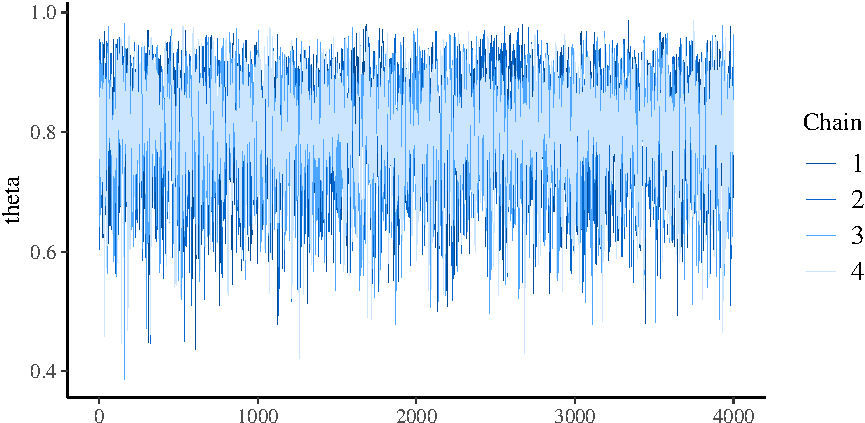
\includegraphics[width=0.8\linewidth]{040_beta_binomial_mod_files/figure-latex/trace-plot-gautret-1} 

}

\caption{Trace-plot per il parametro $\theta$ nel modello Beta-Binomiale.}\label{fig:trace-plot-gautret}
\end{figure}

\noindent
La figura \ref{fig:trace-plot-gautret} mostra che le catene esplorano uno spazio compreso approssimativamenre tra 0.7 e 0.9; tale figura descrive il comportamento \emph{longitudinale} delle catene di Markov.

Possiamo anche esaminare la distribuzione degli stati della catena di Markov, ovvero, dei valori che queste catene visitano lungo il loro percorso, ignorando l'ordine di queste visite. L'istogramma della figura \ref{fig:hist-post-gautret} fornisce una rappresentazione grafica di questa distribuzione per i 16000 valori complessivi delle quattro catene, ovvero per 4000 valori provienienti da ciascuna catena.

\begin{Shaded}
\begin{Highlighting}[]
\FunctionTok{mcmc\_hist}\NormalTok{(stanfit1, }\AttributeTok{pars =} \StringTok{"theta"}\NormalTok{) }\SpecialCharTok{+} 
  \FunctionTok{yaxis\_text}\NormalTok{(}\ConstantTok{TRUE}\NormalTok{) }\SpecialCharTok{+} 
  \FunctionTok{ylab}\NormalTok{(}\StringTok{"count"}\NormalTok{)}
\end{Highlighting}
\end{Shaded}

\begin{figure}[h]

{\centering 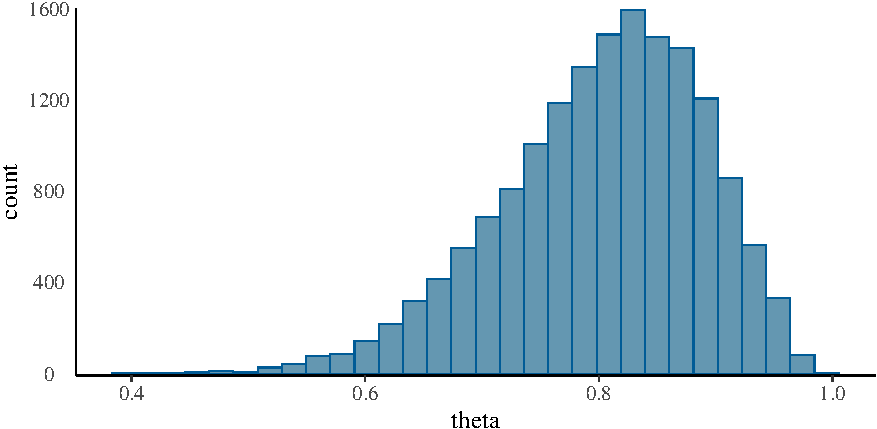
\includegraphics[width=0.8\linewidth]{040_beta_binomial_mod_files/figure-latex/hist-post-gautret-1} 

}

\caption{Istogramma che illustra l'approssimazione della distribuzione a posteriori per il parametro $\theta$ nel modello Beta-Binomiale.}\label{fig:hist-post-gautret}
\end{figure}

Nel modello Beta-Binomiale in cui la verosimiglianza è binomiale con 14 successi su 16 prove e in cui assumiamo una distribuzione a priori di tipo \(\mbox{Beta}(2, 2)\) sul parametro \(\theta\), la distribuzione a posteriori è ancora una distribuzione Beta di parametri \(\alpha\) = 2 + 14 e \(\beta\) = 2 + 16 - 14. La figura \ref{fig:hist-post-gautret-plus-correct} riporta un kernel density plot per i valori delle quattro catene di Markov con sovrapposta in nero la densità \(\mbox{Beta}(16, 4)\). Il punto importante è che la distribuzione dei valori delle catene di Markov produce un'eccellente approssimazione alla distribuzione bersaglio.\footnote{Nel caso presente, il risultato è poco utile dato che è disponibile una soluzione analitica. Tuttavia, questo esercizio mette in evidenza il fatto cruciale che, nei casi in cui possiamo verificarne la soluzione, il campionamento Monte Carlo a catena di Markov è in grado di trovare la risposta corretta. Di conseguenza, possiamo anche essere sicuri che fornirà un'approssimazione alla distribuzione a posteriori anche in quei casi in cui una soluzione analitica non è disponibile.}

\begin{Shaded}
\begin{Highlighting}[]
\FunctionTok{mcmc\_dens}\NormalTok{(stanfit1, }\AttributeTok{pars =} \StringTok{"theta"}\NormalTok{) }\SpecialCharTok{+} 
  \FunctionTok{yaxis\_text}\NormalTok{(}\ConstantTok{TRUE}\NormalTok{) }\SpecialCharTok{+} 
  \FunctionTok{ylab}\NormalTok{(}\StringTok{"density"}\NormalTok{) }\SpecialCharTok{+}
  \FunctionTok{stat\_function}\NormalTok{(}\AttributeTok{fun =}\NormalTok{ dbeta, }\AttributeTok{args =} \FunctionTok{list}\NormalTok{(}\AttributeTok{shape1 =} \DecValTok{16}\NormalTok{, }\AttributeTok{shape2=}\DecValTok{4}\NormalTok{))}
\end{Highlighting}
\end{Shaded}

\begin{figure}[h]

{\centering 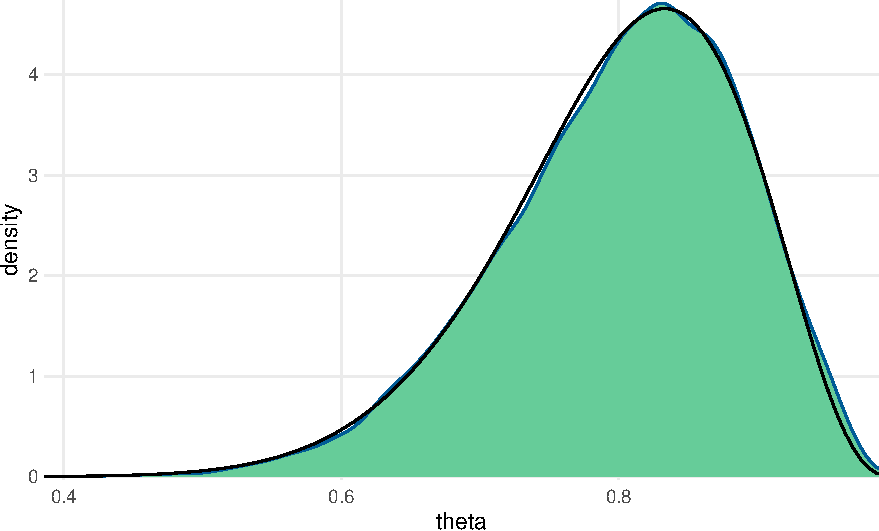
\includegraphics[width=0.8\linewidth]{040_beta_binomial_mod_files/figure-latex/hist-post-gautret-plus-correct-1} 

}

\caption{Istogramma che illustra l'approssimazione della distribuzione a posteriori per il parametro $\theta$ nel modello Beta-Binomiale. La curva nera rappresenta la corretta distribuzione a posteriori Beta(16, 4).}\label{fig:hist-post-gautret-plus-correct}
\end{figure}

Un intervallo di credibilità al 95\% per \(\theta\) si ottiene con la seguente chiamata:

\begin{Shaded}
\begin{Highlighting}[]
\NormalTok{posterior1 }\OtherTok{\textless{}{-}} \FunctionTok{extract}\NormalTok{(stanfit1)}
\NormalTok{rstantools}\SpecialCharTok{::}\FunctionTok{posterior\_interval}\NormalTok{(}\FunctionTok{as.matrix}\NormalTok{(stanfit1), }\AttributeTok{prob =} \FloatTok{0.95}\NormalTok{)}
\CommentTok{\#\textgreater{}                2.5\%    97.5\%}
\CommentTok{\#\textgreater{} theta         0.611   0.9440}
\CommentTok{\#\textgreater{} y\_rep[1]      0.000   1.0000}
\CommentTok{\#\textgreater{} y\_rep[2]      0.000   1.0000}
\CommentTok{\#\textgreater{} y\_rep[3]      0.000   1.0000}
\CommentTok{\#\textgreater{} y\_rep[4]      0.000   1.0000}
\CommentTok{\#\textgreater{} y\_rep[5]      0.000   1.0000}
\CommentTok{\#\textgreater{} y\_rep[6]      0.000   1.0000}
\CommentTok{\#\textgreater{} y\_rep[7]      0.000   1.0000}
\CommentTok{\#\textgreater{} y\_rep[8]      0.000   1.0000}
\CommentTok{\#\textgreater{} y\_rep[9]      0.000   1.0000}
\CommentTok{\#\textgreater{} y\_rep[10]     0.000   1.0000}
\CommentTok{\#\textgreater{} y\_rep[11]     0.000   1.0000}
\CommentTok{\#\textgreater{} y\_rep[12]     0.000   1.0000}
\CommentTok{\#\textgreater{} y\_rep[13]     0.000   1.0000}
\CommentTok{\#\textgreater{} y\_rep[14]     0.000   1.0000}
\CommentTok{\#\textgreater{} y\_rep[15]     0.000   1.0000}
\CommentTok{\#\textgreater{} y\_rep[16]     0.000   1.0000}
\CommentTok{\#\textgreater{} log\_lik[1]   {-}0.493  {-}0.0576}
\CommentTok{\#\textgreater{} log\_lik[2]   {-}0.493  {-}0.0576}
\CommentTok{\#\textgreater{} log\_lik[3]   {-}0.493  {-}0.0576}
\CommentTok{\#\textgreater{} log\_lik[4]   {-}0.493  {-}0.0576}
\CommentTok{\#\textgreater{} log\_lik[5]   {-}0.493  {-}0.0576}
\CommentTok{\#\textgreater{} log\_lik[6]   {-}0.493  {-}0.0576}
\CommentTok{\#\textgreater{} log\_lik[7]   {-}0.493  {-}0.0576}
\CommentTok{\#\textgreater{} log\_lik[8]   {-}0.493  {-}0.0576}
\CommentTok{\#\textgreater{} log\_lik[9]   {-}0.493  {-}0.0576}
\CommentTok{\#\textgreater{} log\_lik[10]  {-}0.493  {-}0.0576}
\CommentTok{\#\textgreater{} log\_lik[11]  {-}0.493  {-}0.0576}
\CommentTok{\#\textgreater{} log\_lik[12]  {-}0.493  {-}0.0576}
\CommentTok{\#\textgreater{} log\_lik[13]  {-}0.493  {-}0.0576}
\CommentTok{\#\textgreater{} log\_lik[14]  {-}0.493  {-}0.0576}
\CommentTok{\#\textgreater{} log\_lik[15]  {-}2.883  {-}0.9436}
\CommentTok{\#\textgreater{} log\_lik[16]  {-}2.883  {-}0.9436}
\CommentTok{\#\textgreater{} lp\_\_        {-}12.734 {-}10.0086}
\end{Highlighting}
\end{Shaded}

Svolgendo un'analisi bayesiana simile a questa, \textcite{Gautret_2020} hanno trovato che gli intervalli di credibilità del gruppo di controllo e del gruppo sperimentale non si sovrappongono. Questo fatto viene interpretato dicendo che il parametro \(\theta\) è diverso nei due gruppi. Sulla base di queste evidenza, \textcite{Gautret_2020} hanno concluso, con un grado di certezza soggettiva del 95\%, che nel gruppo sperimentale vi è una probabilità più bassa di risultare positivi al SARS-CoV-2 rispetto al gruppo di controllo. In altri termini, questa analisi dei dati suggerisce che l'idrossiclorochina sia efficace come terapia per il Covid-19.

\hypertarget{la-critica-di-hulme_2020}{%
\subsection{\texorpdfstring{La critica di \textcite{Hulme_2020}}{La critica di @Hulme\_2020}}\label{la-critica-di-hulme_2020}}

Un articolo pubblicato da \textcite{Hulme_2020} si è posto il problema di rianalizzare i dati di \textcite{Gautret_2020}.\footnote{Si veda \url{https://osf.io/5dgmx/}.} Tra gli autori di questo articolo figura anche Eric-Jan Wagenmakers, uno psicologo molto conosciuto per i suoi contributi metodologici. \textcite{Hulme_2020} hanno osservato che, nelle analisi statistiche riportate, \textcite{Gautret_2020} hanno escluso alcuni dati. Nel gruppo sperimentale, infatti, vi erano alcuni pazienti i quali, anziché migliorare, sono in realtà peggiorati. L'analisi statistica di \textcite{Gautret_2020} ha escluso i dati di questi pazienti. Se consideriamo tutti i pazienti --- non solo quelli selezionati da \textcite{Gautret_2020} --- la situazione diventa la seguente:

\begin{itemize}
\tightlist
\item
  gruppo sperimentale: 10 positivi su 18;
\item
  gruppo di controllo: 14 positivi su 16.
\end{itemize}

L'analisi dei dati proposta da \textcite{Hulme_2020} richiede l'uso di alcuni strumenti statistici che, in queste dispense, non verranno discussi. Ma possiamo giungere alle stesse conclusioni raggiunte da questi ricercatori anche usando le procedure statistiche descritte nel Paragrafo successivo.

\hypertarget{due-proporzioni}{%
\section{Due proporzioni}\label{due-proporzioni}}

Svolgiamo ora l'analisi considerando tutti i dati, come suggerito da \textcite{Hulme_2020}. Per fare questo verrà creato un modello bayesiano per fare inferenza sulla differenza tra due proporzioni. Una volta generate le distribuzioni a posteriori per le proporzioni di ``successi'' nei due gruppi, verrà anche generata la quantità
\[
\omega = \frac{\theta_2 / (1-\theta_2)}{\theta_1 / (1-\theta_1)},
\]
\noindent
ovvero il rapporto tra gli Odds di positività tra i pazienti del gruppo di controllo e gli Odds di positività tra i pazienti del gruppo sperimentale. Se il valore dell'OR è uguale a 1, significa che l'Odds di positività nel gruppo di controllo è uguale all'odds di positività nel gruppo sperimentale, cioè il fattore in esame (somministrazione dell'idrossiclorochina) è ininfluente sulla comparsa della malattia. L'inferenza statistica sull'efficacia dell'idrossiclorochina come terapia per il Covid-19 può dunque essere effettuata esaminando l'intervallo di credibilità al 95\% per l'OR: se tale intervallo include il valore 1, allora non vi è evidenza che l'idrossiclorochina sia efficace come terapia per il Covid-19.

Nell'implementazione di questo modello, la quantità di interesse è dunque l'odds ratio; tale quantità viene calcolata nel blocco \texttt{generated\ quantities} del programma Stan. In questo esempio useremo delle distribuzioni a priori vagamente informative per i parametri \(\theta_1\) e \(\theta_1\).

\begin{Shaded}
\begin{Highlighting}[]
\NormalTok{data\_list }\OtherTok{\textless{}{-}} \FunctionTok{list}\NormalTok{(}
  \AttributeTok{N1 =} \DecValTok{18}\NormalTok{, }
  \AttributeTok{y1 =} \DecValTok{10}\NormalTok{, }
  \AttributeTok{N2 =} \DecValTok{16}\NormalTok{, }
  \AttributeTok{y2 =} \DecValTok{14}
\NormalTok{)}
\end{Highlighting}
\end{Shaded}

\begin{Shaded}
\begin{Highlighting}[]
\NormalTok{modelString }\OtherTok{=} \StringTok{"}
\StringTok{//  Comparison of two groups with Binomial}
\StringTok{data \{}
\StringTok{  int\textless{}lower=0\textgreater{} N1;              // number of experiments in group 1}
\StringTok{  int\textless{}lower=0\textgreater{} y1;              // number of deaths in group 1}
\StringTok{  int\textless{}lower=0\textgreater{} N2;              // number of experiments in group 2}
\StringTok{  int\textless{}lower=0\textgreater{} y2;              // number of deaths in group 2}
\StringTok{\}}
\StringTok{parameters \{}
\StringTok{  real\textless{}lower=0,upper=1\textgreater{} theta1; // probability of death in group 1}
\StringTok{  real\textless{}lower=0,upper=1\textgreater{} theta2; // probability of death in group 2}
\StringTok{\}}
\StringTok{model \{}
\StringTok{  theta1 \textasciitilde{} beta(2, 2);          // prior}
\StringTok{  theta2 \textasciitilde{} beta(2, 2);          // prior}
\StringTok{  y1 \textasciitilde{} binomial(N1, theta1);    // observation model / likelihood}
\StringTok{  y2 \textasciitilde{} binomial(N2, theta2);    // observation model / likelihood}
\StringTok{\}}
\StringTok{generated quantities \{}
\StringTok{  // generated quantities are computed after sampling}
\StringTok{  real oddsratio = (theta2/(1{-}theta2))/(theta1/(1{-}theta1));}
\StringTok{\}}
\StringTok{"}
\FunctionTok{writeLines}\NormalTok{(modelString, }\AttributeTok{con =} \StringTok{"code/twoprop1.stan"}\NormalTok{)}
\end{Highlighting}
\end{Shaded}

\begin{Shaded}
\begin{Highlighting}[]
\NormalTok{file }\OtherTok{\textless{}{-}} \FunctionTok{file.path}\NormalTok{(}\StringTok{"code"}\NormalTok{, }\StringTok{"twoprop1.stan"}\NormalTok{)}
\end{Highlighting}
\end{Shaded}

\begin{Shaded}
\begin{Highlighting}[]
\NormalTok{mod }\OtherTok{\textless{}{-}} \FunctionTok{cmdstan\_model}\NormalTok{(file)}
\end{Highlighting}
\end{Shaded}

\begin{Shaded}
\begin{Highlighting}[]
\NormalTok{fit }\OtherTok{\textless{}{-}}\NormalTok{ mod}\SpecialCharTok{$}\FunctionTok{sample}\NormalTok{(}
  \AttributeTok{data =}\NormalTok{ data\_list,}
  \AttributeTok{iter\_sampling =}\NormalTok{ 4000L,}
  \AttributeTok{iter\_warmup =}\NormalTok{ 2000L,}
  \AttributeTok{seed =}\NormalTok{ SEED,}
  \AttributeTok{chains =}\NormalTok{ 4L,}
  \AttributeTok{parallel\_chains =}\NormalTok{ 4L,}
  \AttributeTok{refresh =} \DecValTok{0}\NormalTok{,}
  \AttributeTok{thin =} \DecValTok{1}
\NormalTok{)}
\end{Highlighting}
\end{Shaded}

\begin{Shaded}
\begin{Highlighting}[]
\NormalTok{stanfit }\OtherTok{\textless{}{-}}\NormalTok{ rstan}\SpecialCharTok{::}\FunctionTok{read\_stan\_csv}\NormalTok{(fit}\SpecialCharTok{$}\FunctionTok{output\_files}\NormalTok{())}
\end{Highlighting}
\end{Shaded}

\begin{Shaded}
\begin{Highlighting}[]
\FunctionTok{print}\NormalTok{(}
\NormalTok{  stanfit,}
  \AttributeTok{pars =} \FunctionTok{c}\NormalTok{(}\StringTok{"theta1"}\NormalTok{, }\StringTok{"theta2"}\NormalTok{, }\StringTok{"oddsratio"}\NormalTok{),}
  \AttributeTok{digits\_summary =}\NormalTok{ 3L}
\NormalTok{)}
\CommentTok{\#\textgreater{} Inference for Stan model: twoprop1{-}202112300706{-}1{-}608003.}
\CommentTok{\#\textgreater{} 4 chains, each with iter=6000; warmup=2000; thin=1; }
\CommentTok{\#\textgreater{} post{-}warmup draws per chain=4000, total post{-}warmup draws=16000.}
\CommentTok{\#\textgreater{} }
\CommentTok{\#\textgreater{}            mean se\_mean    sd  2.5\%   25\%   50\%   75\%  97.5\% n\_eff}
\CommentTok{\#\textgreater{} theta1    0.546   0.001 0.104 0.337 0.475 0.547 0.619  0.743 11214}
\CommentTok{\#\textgreater{} theta2    0.801   0.001 0.087 0.605 0.747 0.812 0.865  0.939 12359}
\CommentTok{\#\textgreater{} oddsratio 4.859   0.049 4.740 0.914 2.221 3.599 5.933 16.251  9207}
\CommentTok{\#\textgreater{}           Rhat}
\CommentTok{\#\textgreater{} theta1       1}
\CommentTok{\#\textgreater{} theta2       1}
\CommentTok{\#\textgreater{} oddsratio    1}
\CommentTok{\#\textgreater{} }
\CommentTok{\#\textgreater{} Samples were drawn using NUTS(diag\_e) at Gio Dic 30 07:06:01 2021.}
\CommentTok{\#\textgreater{} For each parameter, n\_eff is a crude measure of effective sample size,}
\CommentTok{\#\textgreater{} and Rhat is the potential scale reduction factor on split chains (at }
\CommentTok{\#\textgreater{} convergence, Rhat=1).}
\end{Highlighting}
\end{Shaded}

L'intervallo di credibilità del 95\% per l'OR include il valore di 1.0 (ovvero, il valore che indica che gli odds di positività sono uguali nei due gruppi). In base agli standard correnti, un risultato di questo tipo non viene considerato come evidenza sufficiente per potere concludere che il parametro \(\theta\) assume un valore diverso nei due gruppi. In altri termini, se consideriamo tutti i dati, e non solo quelli selezionati dagli autori della ricerca originaria, non vi è evidenza alcuna che l'idrossiclorochina sia efficace come terapia per il Covid-19.

\hypertarget{considerazioni-conclusive}{%
\section*{Considerazioni conclusive}\label{considerazioni-conclusive}}
\addcontentsline{toc}{section}{Considerazioni conclusive}

Concludiamo questa discussione dicendo che ciò che è stato presentato in questo capitolo è un esercizio didattico: la ricerca di \textcite{Gautret_2020} include tante altre informazioni che non sono state qui considerate. Tuttavia, notiamo che la semplice analisi statistica che abbiamo qui descritto è stata in grado di replicare le conclusioni a cui sono giunti (per altra via) \textcite{Hulme_2020}.


% Bibliography
%%%%%%%%%%%%%%%%%%%%%%%%%%%%%%%%%%%%%%%%%%%%%%%%%%%%%%%%%%

\backmatter
\SmallMargins

\printbibliography
\onecolumn


% Tables (of tables, of figures)
%%%%%%%%%%%%%%%%%%%%%%%%%%%%%%%%%%%%%%%%%%%%%%%%%%%%%%%%%%


\cleardoublepage
\LargeMargins
\listoffigures


% After-body (LaTeX code inclusion)
%%%%%%%%%%%%%%%%%%%%%%%%%%%%%%%%%%%%%%%%%%%%%%%%%%%%%%%%%%




% Back cover
%%%%%%%%%%%%%%%%%%%%%%%%%%%%%%%%%%%%%%%%%%%%%%%%%%%%%%%%%%%

% Even page, small margins, no running head, no page number.
\evenpage
\SmallMargins
\thispagestyle{empty}

\begin{normalsize}

\begin{description}

\selectlanguage{italian}
\item[Abstract]
This document contains the material of the lessons of Psicometria B000286 (2021/2022) aimed at students of the first year of the Degree Course in Psychological Sciences and Techniques of the University of Florence, Italy.
\item[Keywords]
Data science, Bayesian statistics.
~\\

\end{description}

\end{normalsize}


\end{document}
